\chapter{Work Progress}
\label{chap:work}
\setlength{\parskip}{1.5mm}
%\setlength{\baselineskip}{1.4mm}
\section{Verifying the Algorithm in MATLAB}
\subsection{Model of Non-Linear Dynamic System}
A schematic diagram of the compound triple-pendulum system is shown in Figure 5.1.The bars of the pendulum have significant mass so that it can be modeled as a compound pendulum. The model has been parameterized according to the physical characteristics of the system including mass of the bars, their inertia etc. 
% Damping factors were also included in the model for higher degree of chaos and non-linearity in the system. 
% Each bar ${i}$ is defined by a set of four parameters: 
% ${I_{i}}$, the moment of inertia of the bar, ${m_{i}}$, the mass of the bar,
%  ${L_{i}}$, the length of the bar, and
%  ${k_{i}}$, the damping coefficient of the bar rotating about it’s upper joint. 
The position and velocity of the bars are defined by the six system state variables: $\theta$\textsubscript{1}, $\theta$\textsubscript{2}, $\theta$\textsubscript{3}, ${\dot{\theta\textsubscript{1}}}$, ${\dot{\theta\textsubscript{2}}}$, ${\dot{\theta\textsubscript{3}}}$

%\begin{figure}
%\centering
%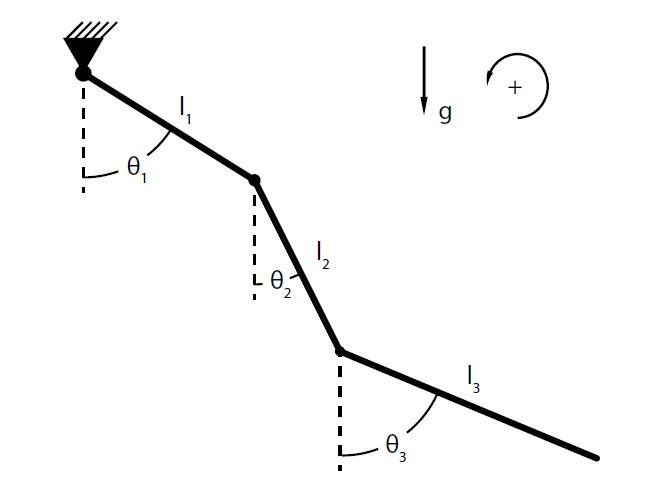
\includegraphics[width=8cm]{pendulum.jpg}
%\caption{Schematic Diagram of Triple Pendulum System}\label{fig:pendulum}
%\end{figure}
% 

\begin{figure}[H]
\begin{subfigure}{0.5\textwidth}
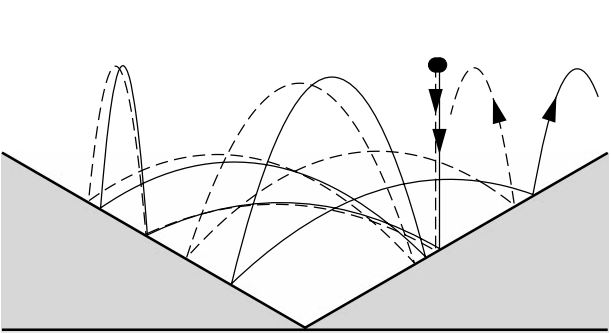
\includegraphics[width=1.1\linewidth]{ball.jpg}
\caption{Chaotic motion of a bouncing ball}\label{fig:ball}
\end{subfigure}
\begin{subfigure}{0.5\textwidth}
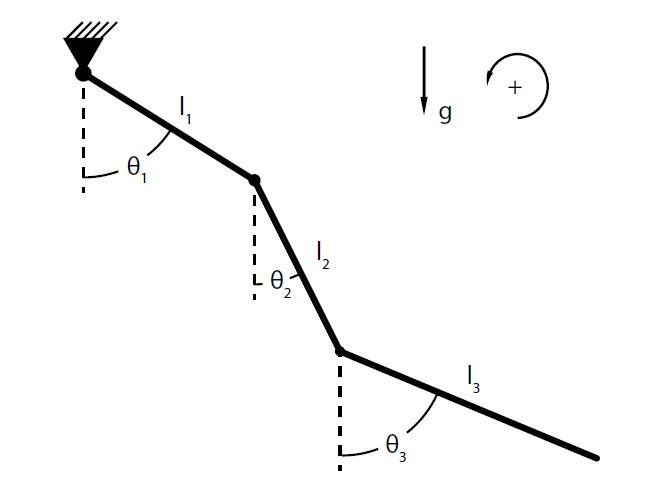
\includegraphics[width=0.8\linewidth]{pendulum.jpg}
\caption{Schematic Diagram of Triple Pendulum}\label{fig:pendulum}
\end{subfigure}
\caption{Examples of Non-Linear Dynamic systems}\label{fig:image1}

\end{figure}
\begin{figure}[h]
\begin{subfigure}{0.5\textwidth}
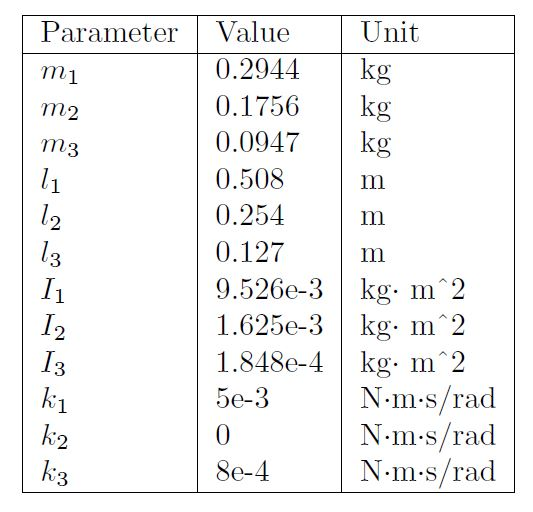
\includegraphics[width=0.8\linewidth]{param.jpg}
\caption{Table 1}\label{fig:param}
\end{subfigure}
\begin{subfigure}{0.5\textwidth}
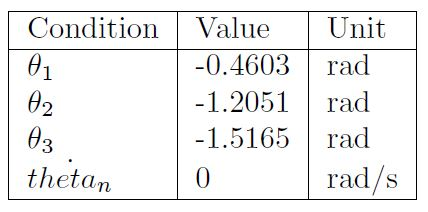
\includegraphics[width=0.8\linewidth]{ic.jpg}
\caption{Table 2}\label{fig:ic}
\end{subfigure}
\caption{Parameters \& Initial Conditions for the Initial Value Problem}\label{fig:image2}
\end{figure}

% \begin{figure}
% 
% 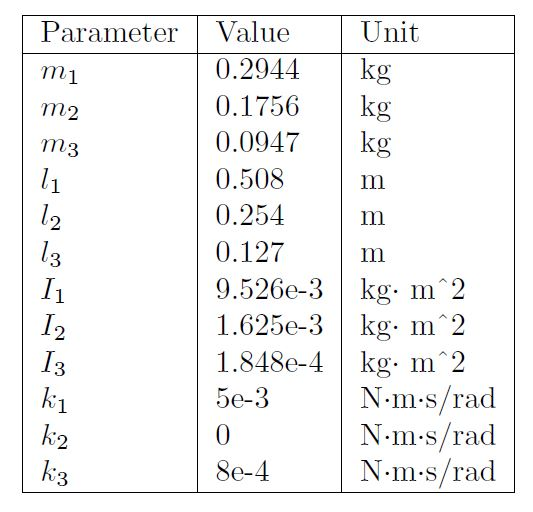
\includegraphics[width=8cm]{param.jpg}
% \caption{Parametric Values used for Simulation}\label{fig:param}
% \end{figure}
% 
% \begin{figure}
% % \centering
% 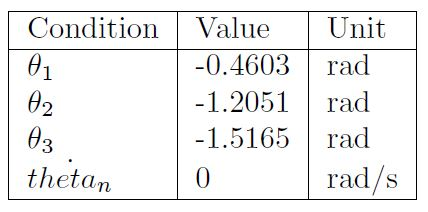
\includegraphics[width=8cm]{ic.jpg}
% \caption{Initial Conditions used for Simulation}\label{fig:ic}
% \end{figure}

\subsection{Simulation of Compound Triple Pendulum}
This compound triple-pendulum model has been simulated using MATLAB using approximate differential equations describing the random motions. The parameters and initial conditions of the ODEs are given in Table 1 and Table 2 respectively. For the simulation, simple numerical methods were used to solve the differential equations and the values corresponding to the angular position of the bars were obtained within a certain duration of time with a predefined precision. This generates the mapping values for the encryption module. 

% \begin{figure}[H]
% \centering
% 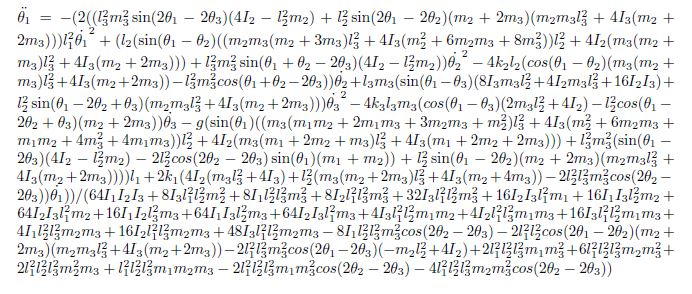
\includegraphics[width=16cm]{diff1.jpg}
% \caption{Differential Equation for ${\theta\textsubscript{1}}$}\label{fig:diff1}
% \end{figure}
% 
% 
% \begin{figure}[H]
% \centering
% 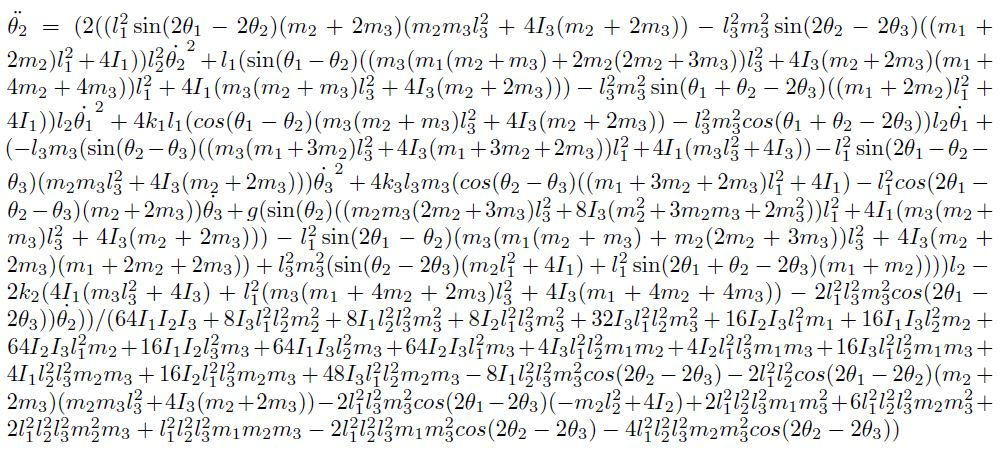
\includegraphics[width=16.5cm]{diff2.jpg}
% \caption{Differential Equation for ${\theta\textsubscript{2}}$}\label{fig:diff2}
% \end{figure}
% 
% 
% \begin{figure}[H]
% \centering
% 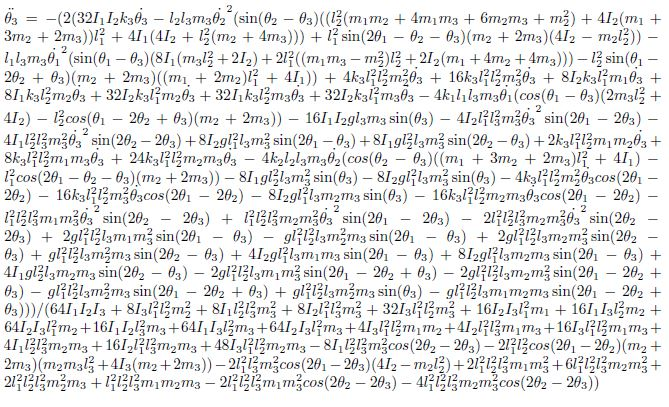
\includegraphics[width=16.5cm]{diff3.jpg}
% \caption{Differential Equation for ${\theta\textsubscript{3}}$}\label{fig:diff3}
% \end{figure}
% \vfill
\subsubsection{Simulation Results}
These are some of the observations from the simulation of the triple-pendulum model for a duration of t = 0 to t = 10 seconds with $\Delta$t = 0.001 :\\
(i) Initial conditions are same as given in Table 1 \& 2:\\
 
\begin{figure}[H]
\begin{subfigure}{0.5\textwidth}
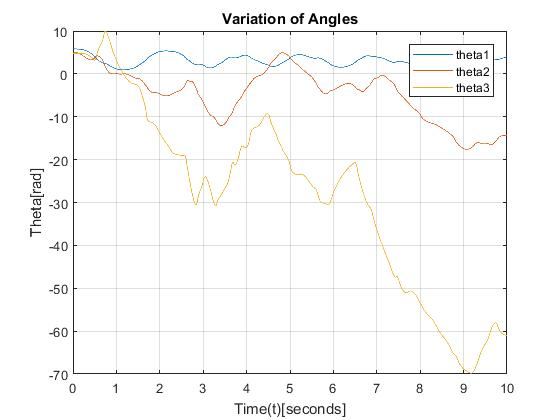
\includegraphics[width=1\linewidth]{theta.jpg}
\caption{Plot of ${\theta}$ vs Time}\label{fig:theta}
\end{subfigure}
\begin{subfigure}{0.5\textwidth}
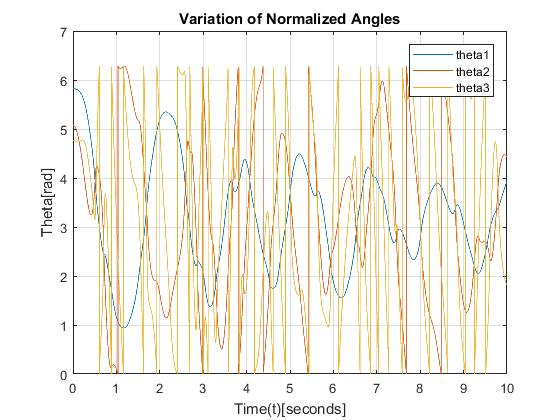
\includegraphics[width=1\linewidth]{theta_norm.jpg}
\caption{Plot of Normalized ${\theta}$ vs Time}\label{fig:theta_norm}
\end{subfigure}
\caption{Motion of Triple-Pendulum for t = 0 to t = 10 sec}\label{fig:image3}
\end{figure}

\begin{figure}[H]
\centering
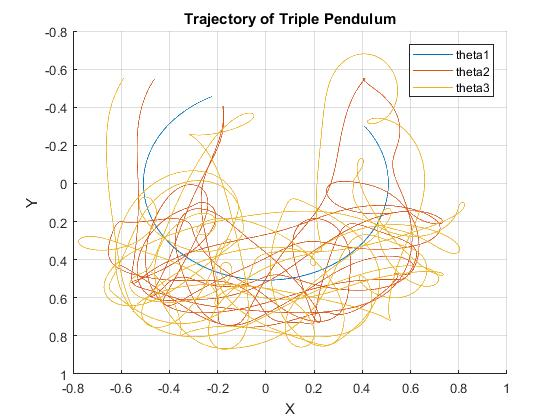
\includegraphics[width=0.7\linewidth]{trajectory.jpg}
\caption{Plot of Motion of Triple-Pendulum}\label{fig:trajectory}
\end{figure}


\subsection{Encryption - Decryption}
Our approach is to convert the plain-text into ascii format and  map the value to the partitioned intervals of the triple-pendulum motion simulated within a specific duration of time for a particular set of parameters and initial conditions. The initial conditions and parameters of the different equation forms a part of the private key. Following the Baptista-type method, the entire range of the chaotic function was partitioned into a number of intervals equal to the number of characters. Each character in the plain-text is then mapped to a specific interval and then to a time point randomly selecting from that interval.  

\begin{figure}[H]
\centering
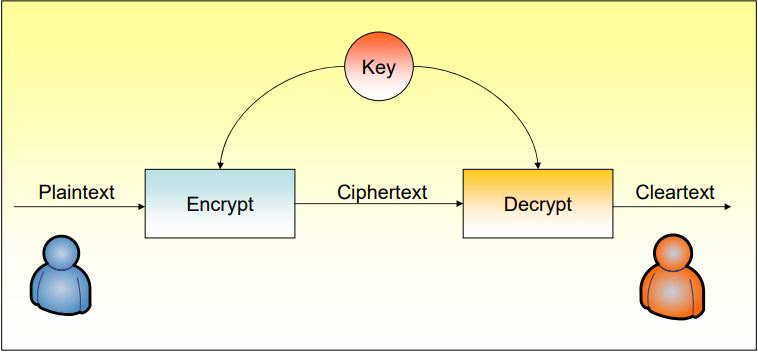
\includegraphics[width=10cm]{crypto.jpg}
\caption{Working Principle of a Symmetric Cryptosystem}\label{fig:crypto}
\end{figure}

On the decryption module, the interval in which the encrypted value lies is computed from the generated motion of the triple-pendulum for the same key and the corresponding index would then refer to the ascii converted clear-text. Converting them into characters, the message can be decoded.\\
\begin{figure}[H]
\centering
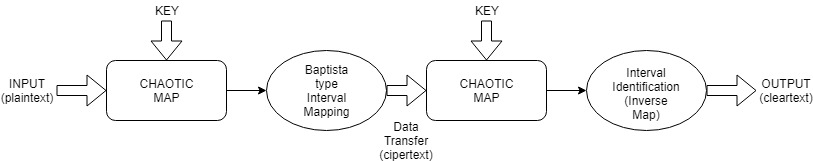
\includegraphics[width=16cm]{Dataflow.jpg}
\caption{Encryption-Decryption Strategy}\label{fig:Dataflow}
\end{figure}


\section{Key Generation}
It is observed that for certain specific parameters or initial conditions, the motion of the bars of the triple-pendulum shows periodic nature after a certain span of time. Hence there is a need to eliminate those parameters or initial conditions for which the motion is periodic as the periodic nature breaks the chaotic behavior of the system. For that a test for periodicity was employed to extract the prominent period of the signal using statistical analysis on the spectrum of the signal. The test used is known as {\bf{\em Fisher's g-statistic test}}(see [11]). This method is based on the test of significance of the periodic components of the signal derived from its periodogram. 

\begin{figure}[H]
\centering
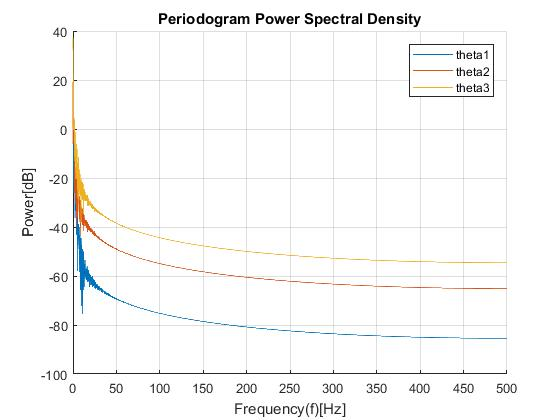
\includegraphics[width=0.7\linewidth]{periodogram.jpg}
\caption{Periodogram Plot for ${\theta}$}\label{fig:periodogram}
\end{figure}


\begin{figure}[H]
\begin{subfigure}{0.5\textwidth}
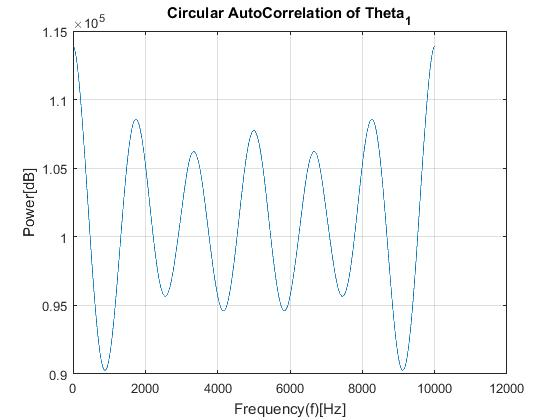
\includegraphics[width=1\linewidth]{auto_corr1.jpg}
\caption{Plot of Circular Auto-Correlation for ${\theta_{1}}$}\label{fig:cir_auto1}
\end{subfigure}
\begin{subfigure}{0.5\textwidth}
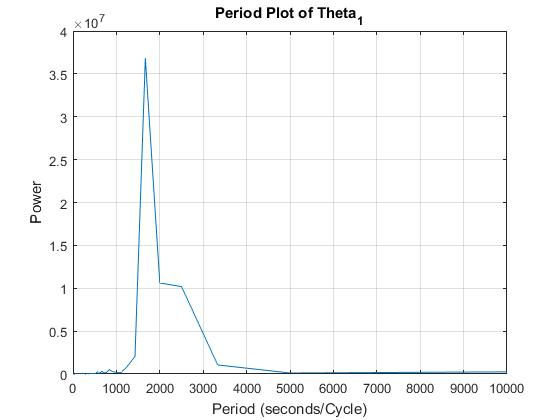
\includegraphics[width=1\linewidth]{period1.jpg}
\caption{Plot of Periodicity for ${\theta_{1}}$}\label{fig:period1}
\end{subfigure}
\caption{Periodic Properties of ${\theta_{1}}$}\label{fig:image4}
\end{figure}

\begin{figure}[H]
\begin{subfigure}{0.5\textwidth}
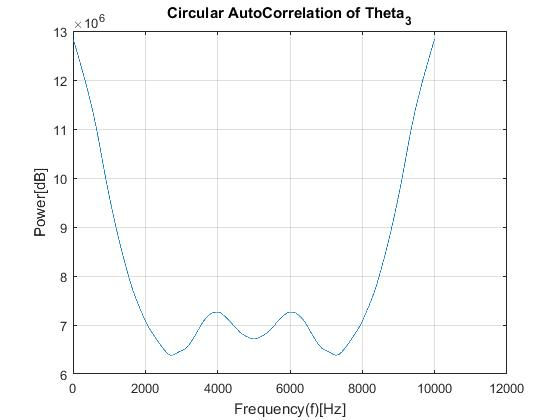
\includegraphics[width=1\linewidth]{auto_corr3.jpg}
\caption{Plot of Circular Auto-Correlation for ${\theta_{3}}$}\label{fig:cir_auto3}
\end{subfigure}
\begin{subfigure}{0.5\textwidth}
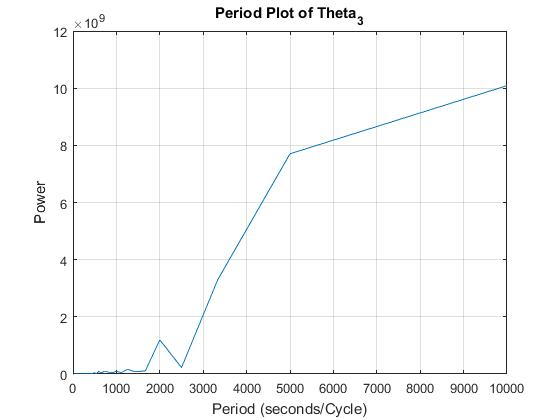
\includegraphics[width=1\linewidth]{period3.jpg}
\caption{Plot of Periodicity for ${\theta_{3}}$}\label{fig:period3}
\end{subfigure}
\caption{Periodic Properties of ${\theta_{3}}$}\label{fig:image5}
\end{figure}

From the figures 5.8 \& 5.9 , it is observed that there is peak at 1700 (seconds/Cycle) for $\theta_{1}$ whereas no such peak occurs for $\theta_{3}$. Thus $\theta_{1}$ is periodic in nature. The values obtained from the periodicity test and plots of circular auto-correlation clearly differentiates the parameters and initial values which leads to periodic nature of the motion and those which lead to non-periodic nature of the motion. Thus by iterating through all possibles values of the parameters and checking likewise for non-periodic nature, a set of keys was generated and stored. 


\section{FPGA Implementation}
The complete design is being implemented at Register-Transfer Level (RTL) in {\bf Verilog HDL} and the target device chosen is Digilent Nexys Board with {\bf Xilinx Artix-7 FPGA}. The following diagram shows the implementation plan for the design :
\begin{figure}[H]
\centering
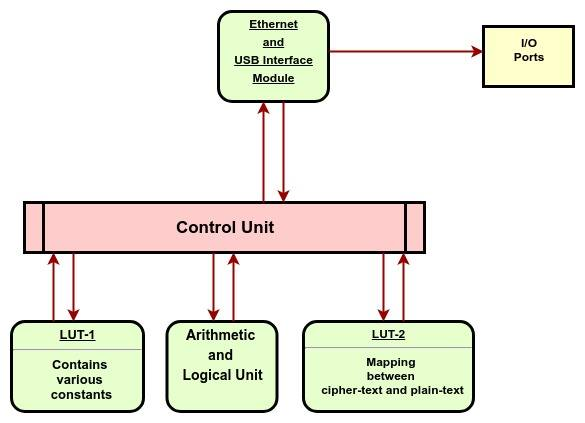
\includegraphics[width=10cm]{fpga_block.jpg}
\caption{Block Diagram of FPGA Implementation}\label{fig:fpga_block}
\end{figure}

1. {\bf Arithmetic and Logical Unit (ALU)} - The ALU uses floating-point arithmetic whose precision can be configured at the time of synthesis. This has been done to enable the study of how security strength varies with arithmetic precision.

2. {\bf Look-Up Table (LUT)} - A fast Look-Up table is to be implemented for storing various constants and the mapping between clear-text and cipher-text.

3. {\bf Ethernet and USB Module} - These are required to enable the device to encrypt or decrypt both a stream of data as well as complete file.

4. {\bf Control Unit} - Essentially a state machine that co-ordinates the operation of all other modules including evaluation of state-variables and transfer of data through USB/Ethernet port.

\section{Analysis}
\subsection{General Properties of the Cryptosystem}
\subsubsection{Test for Chaos}
There are some essential requirements that need to be obeyed by any chaos based cryptosystem. These requirements include:
\begin{enumerate}
	\item Sensitivity to Parametric values: A small variation in one of the system parameters is enough to make two trajectories, starting at the same initial point, separate at exponential rate.
	\item Sensitivity to Initial  Condition:  two  trajectories  starting  at  two  different,  though  arbitrarily  close,  initial points separate from each other exponentially.
	\item Ergodicity:  Almost every trajectory tends to an invariant distribution that is independent of the initial conditions, and almost every trajectory will eventually visit any arbitrary interval of arbitrary size.
\end{enumerate}

\begin{figure}[H]
\begin{subfigure}{0.5\textwidth}
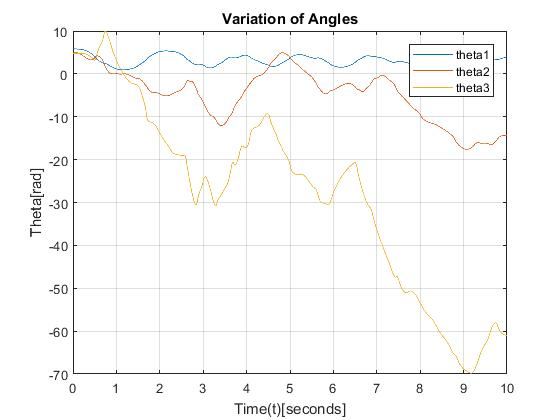
\includegraphics[width=1\linewidth]{theta.jpg}
\caption{Variation of ${\theta}$ for ${m_{1}=0.2944}$}\label{fig:theta_comp}
\end{subfigure}
\begin{subfigure}{0.5\textwidth}
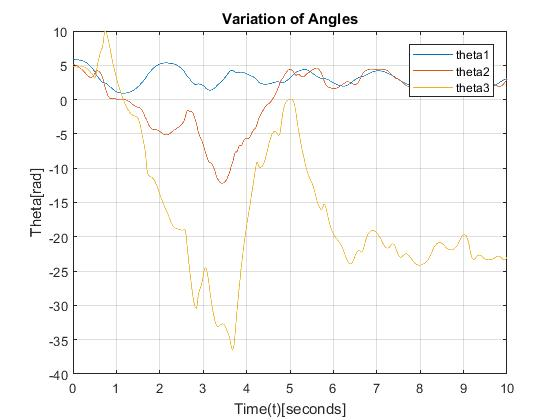
\includegraphics[width=1\linewidth]{theta_near.jpg}
\caption{Variation of ${\theta}$ for ${m_{1}=0.294401}$}\label{fig:trajectory_near_comp}
\end{subfigure}
\caption{Plot showing Sensitivity to Parameter value ${m}$ with ${\Delta m = 10^{-6}}$}\label{fig:image6}
\end{figure}

\begin{figure}[H]
\begin{subfigure}{0.5\textwidth}
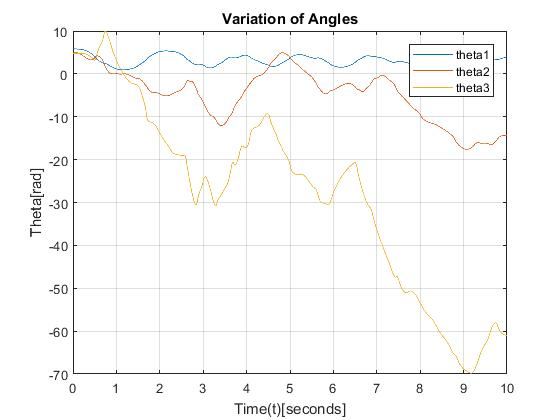
\includegraphics[width=1\linewidth]{theta.jpg}
\caption{Variation of ${\theta}$ for ${\theta_{1}(0)=-0.4603}$}\label{fig:theta_comp}
\end{subfigure}
\begin{subfigure}{0.5\textwidth}
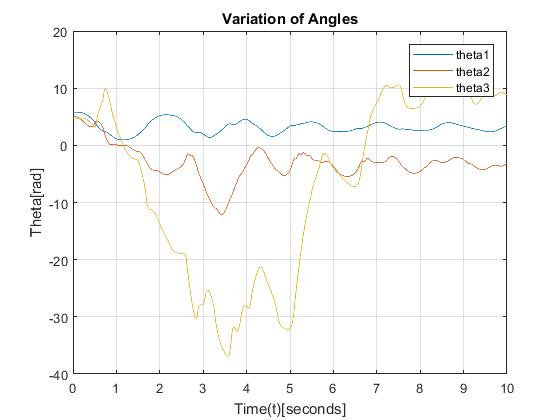
\includegraphics[width=1\linewidth]{theta_ch.jpg}
\caption{Variation of ${\theta}$ for ${\theta_{1}(0)=-0.460301}$}\label{fig:theta_ch_comp}
\end{subfigure}
\caption{Plot showing Sensitivity to Intital condition of ${\theta_{1}}$with ${\Delta \theta_{1} = 10^{-6}}$}\label{fig:image7}
\end{figure}

The proposed cryptosystem also holds such properties. The three qualities mentioned earlier are clearly evident from the plots and graphs shown Fig. 5.11 and Fig. 5.12. It is observed that keeping the parameters in one case and initial conditions in another case, constant leads to two completely different trajectories. Thus the map generated from the compound triple pendulum model possesses the essential chaotic properties to be employed in a general cryptosystem. 

\subsubsection{Collision Test}
Collision resistance is a property of cryptographic algorithms which makes it difficult to find two inputs which are encrypted to the same output. It must be ensured that finding collisions must be kept as hard as some of the hard mathematical problems like integer factorization  or discrete logarithm. Collision resistance does not mean that no collisions exist; simply that they are hard to find. Here, we show that the proposed algorithm is fully collision resistant i.e. no collisions exist.

Since the entire range of $\theta$'s are partitioned according to the number of characters(say 256), different characters are mappped to points in different intervals. Hence two different inputs having different characters are completely mapped to different intervals. So the encryption scheme is completely free of collisions. 

\subsubsection{Test for Randomness}
For testing randomness of the chaotic map, statistical tests are generally applied. These statistical tests are generally employed for testing randomness in pseudo random number generators. Here, Diehard random number generator test suite has been employed to do such tests. Developed by George Marsaglia, Diehard is a battery of tests which are used to determine the quality of PRNGs. The list of tests performed on the generated chaotic map data and the corresponding results obtained are shown in Table 5.1.

\begin{table}[h!]
\begin{center}
\caption{Dieharder Test}
\label{tab:table1}
\begin{tabular}{|c|c|c|c|c|c|} % <-- Alignments: 1st column left, 2nd middle and 3rd right, with vertical lines in between
    \hline
    \textbf{test\_name} & \textbf{ntup} & \textbf{tsamples} & \textbf{psamples} & \textbf{p-value} & \textbf{Assessment}\\
    \hline
    diehard\_birthdays &    0 &        100 &      100 & 0.98409924 &   PASSED \\  
    diehard\_operm5 &    0 &    1000000 &      100 & 0.02570841 &   PASSED \\  
    diehard\_rank\_32x32 &    0 &      40000 &      100 & 0.30314396 &   PASSED \\  
    diehard\_rank\_6x8 &    0 &     100000 &      100 & 0.07586247 &   PASSED \\  
    diehard\_bitstream &    0 &    2097152 &      100 & 0.83264505 &   PASSED \\  
    diehard\_opso &    0 &    2097152 &      100 & 0.93701062 &   PASSED \\  
    diehard\_oqso &    0 &    2097152 &      100 & 0.63759752 &   PASSED \\  
    diehard\_dna &    0 &    2097152 &      100 & 0.73795350 &   PASSED \\  
    diehard\_count\_1s\_str &    0 &     256000 &      100 & 0.77268562 &   PASSED \\  
    diehard\_count\_1s\_byt &    0 &     256000 &      100 & 0.55542008 &   PASSED \\  
    diehard\_parking\_lot &    0 &      12000 &      100 & 0.70977074 &   PASSED \\  
    diehard\_2dsphere &    2 &       8000 &      100 & 0.58428028 &   PASSED \\  
    diehard\_3dsphere &    3 &       4000 &      100 & 0.86446205 &   PASSED \\  
    diehard\_squeeze &    0 &     100000 &      100 & 0.19422339 &   PASSED \\  
    diehard\_sums &    0 &        100 &      100 & 0.33263813 &   PASSED \\  
    diehard\_runs &    0 &     100000 &      100 & 0.50609448 &   PASSED \\    
    diehard\_craps &    0 &     200000 &      100 & 0.36377661 &   PASSED \\   
    marsaglia\_tsang\_gcd &    0 &   10000000 &      100 & 0.66121444 &   PASSED \\ 
    sts\_monobit &    1 &     100000 &      100 & 0.31074688 &   PASSED \\  
    sts\_runs &    2 &     100000 &      100 & 0.98606705 &   PASSED \\  
    sts\_serial &    1 &     100000 &      100 & 0.23629469 &   PASSED \\  
    sts\_serial &    2 &     100000 &      100 & 0.85410639 &   PASSED \\  
    sts\_serial &    8 &     100000 &      100 & 0.11131795 &   PASSED \\  
    sts\_serial &   16 &     100000 &      100 & 0.83380616 &   PASSED \\  
    rgb\_bitdist &    1 &     100000 &      100 & 0.45061356 &   PASSED \\  
    rgb\_bitdist &    6 &     100000 &      100 & 0.53111009 &   PASSED \\   
    rgb\_bitdist &   12 &     100000 &      100 & 0.64865649 &   PASSED \\  
    rgb\_minimum\_distance &    2 &      10000 &     1000 & 0.41755433 &   PASSED \\   
    rgb\_minimum\_distance &    4 &      10000 &     1000 & 0.11298477 &   PASSED \\  
    rgb\_permutations &    2 &     100000 &      100 & 0.79654377 &   PASSED \\ 
    rgb\_permutations &    4 &     100000 &      100 & 0.85371565 &   PASSED \\  
    rgb\_lagged\_sum &    0 &    1000000 &      100 & 0.92039997 &   PASSED \\   
    rgb\_lagged\_sum &   16 &    1000000 &      100 & 0.78219023 &   PASSED \\   
    rgb\_lagged\_sum &   32 &    1000000 &      100 & 0.64955712 &   PASSED \\  
    rgb\_kstest\_test &    0 &      10000 &     1000 & 0.58005862 &   PASSED \\  
    dab\_bytedistrib &    0 &   51200000 &        1 & 0.01089458 &   PASSED \\  
    dab\_dct &  256 &      50000 &        1 & 0.06122408 &   PASSED \\  
    dab\_filltree &   32 &   15000000 &        1 & 0.12524761 &   PASSED \\   
    dab\_filltree2 &    0 &    5000000 &        1 & 0.50605989 &   PASSED \\  
    dab\_monobit2 &   12 &   65000000 &        1 & 0.27940682 &   PASSED \\  
        
    \hline
\end{tabular}
\end{center}
\end{table}

It is observed that in most of the tests, the chaotic map generator performs well. This can be attributed largely due to the non-linear dynamics of the map.

\subsection{Complexity Analysis}

In this report, we give an overview of the computational complexity of the algorithm both on software as well as hardware level.

\subsubsection{Algorithm Complexity}
Firstly, the computation of the state variable (${\theta}$) values for a time duration $t$ and time step $\Delta t$ requires $N$ iterations where $N= \frac{t}{\Delta t}$. In each iteration only 6 equations are solved for the 6 state variables ($\theta_{1}, \theta_{2}, \theta_{3}, \dot{\theta_{1}}, \dot{\theta_{2}}, \dot{\theta_{3}}$) each in $O(1)$ time. Thus the time required for generating the map is asymptotically $O(N)$. Here space complexity is also $O(N)$ for storing the state variable values. Secondly, Baptista type patitioning takes constant time if the range of the variables are already computed in the previous step. For assigning the variable values to the corresponding intervals, $O(N)$ time is required for each value. Thirdly, for encryption of a plaintext having $M$ characters, there would be $M$ iterations and in each iteration the encrypted value is randomly selected from the computed interval which takes constant time. So overall time complexity of encryption is $O(N+M)$. Space complexity is still $O(N)$. Similarly, for decryption time complexity is also $O(N+M)$.\\
\textbf{Information Rate:} The information rate of any cryptosysytem is define d as the ratio of the size of plaintext to that of the cipher text. In our cryptosystem, we have
\begin{equation}
R = \frac{plaintext\ size}{ciphertext\ size} = \frac{8*M}{\log_2N*M} = \frac{8}{\log_2N}
\end{equation}
\subsubsection{Hardware Complexity}
